\chapter{Hinweise zur Installation, \"Ubersetzung und zum Ausdrucken}


\section{Verwendung von TeXShop (Apple-Welt)}

Unter den ausgelieferten Dateien befinden sich zwei \textbf{engine}-Dateien: 

\begin{seList}
\item \verb+dhbw-wa.engine+
\item \verb+dhbw-wa-remove-all.engine+ (l\"oscht alle erzeugten \textsl{Hilfsdateien})
\end{seList}

Mit jeder dieser beiden Dateien kann man z. B. die Vorlage\newline
\hspace*{\fill}\texttt{\seVorlage.tex}\hspace*{\fill}\newline
\"ubersetzen. Alle Verzeichnisse (insbesondere Abk\"urzungs- und Symbolverzeichnis) 
sowie das Glossar werden (hoffentlich) korrekt erstellt.  

In den engine-Dateien ist beschrieben, an welcher Stelle sie im Mac OS X Dateisystem 
installiert werden m\"ussen, damit man sie direkt von TeXShop aus aufrufen kann. 

\section{Verwendung von MiKTeX (Windows-Welt)}

\subsection{Batch-Dateien zur \"Ubersetzung des \LaTeX-Dokuments}

F\"ur die \"Ubersetzung wird eine Batch-Datei \verb+make-wa.bat+ zur Verf\"ugung 
gestellt, mit der man in der Windows-\textsl{Eingabeaufforderung} (cmd) z. B. die Vorlage \"ubersetzen kann. 

Der Aufruf lautet: \texttt{make-wa.bat \seVorlage}

Hierbei ist zu beachten, dass die Dateiendung \texttt{.tex} \textbf{NICHT} angegeben werden darf.

Alternativ kann die Batch-Datei \verb+make-wa-remove-all.bat+ verwendet werden, die alle erzeugten 
Hilfsdateien l\"oscht.




Da MiKTeX eine andere Version von \verb+jurabib+ verwendet, mit der sich die 
Vorlage nicht korrekt \"ubersetzen l\"asst, werden die beiden Dateien 

\begin{seList}
\item \verb+jurabib.sty+ und 
\item \verb+jurabib.bst+
\end{seList}

aus der TeX Live Version von Mac OS X mitgeliefert. Damit sollte die 
\"Ubersetzung problemlos funktionieren. 

\subsection{Installation und Konfiguration von TeXworks}

Obwohl TeXworks ein Bestandteil der MiKTeX-Distribution ist, empfiehlt es sich, 
TeXworks von der Seite \url{http://www.tug.org/texworks} herunterzuladen und 
neu zu installieren. Damit lassen sich -- zumindest unter Windows XP -- z. B. die Eintr\"age 
ins Startmen\"u oder auch ein Icon auf dem Desktop leicht erzeugen.   

Die Batch-Dateien f\"ur die pdf-Erzeugung sind wie folgt in TeXworks integrierbar\footnote{Der Hinweis f\"ur die 
Konfiguration stammt von Marc de Vries -- vielen Dank.}:

\begin{seList}
\item
Im Men\"u \textsl{Bearbeiten $\rightarrow$ Einstellungen} den Reiter \textsl{Textsatz} ausw\"ahlen.
\item 
Im unteren Bereich \textsl{Verarbeitungsprogramme} auf das \textsl{+} klicken.
\item
Im aufgerufenen Dialog \textsl{Konfiguration Textsatz} unter \textsl{Name:} einen passenden 
Namen eingeben, z. B. \texttt{seWA}.
\item
Bei \textsl{Befehl/Datei:} auf \textsl{Durchsuchen} klicken und die \texttt{.bat}-Datei \newline 
\hspace*{\fill} -- z. B. \texttt{make-wa-remove-all.bat} -- \hspace*{\fill}\newline 
         ausw\"ahlen. 
\item
Bei \textsl{Argumente:} auf das \textsl{+} klicken und \texttt{\$basename} eingeben (siehe \vref{texworks}).
\item
Mit \textsl{OK} best\"atigen und gegebenenfalls im Reiter \textsl{Textsatz} unter \textsl{Standard:} 
\texttt{seWA} ausw\"ahlen.         
\end{seList}

Durch das Anklicken des kleinen gr\"unen Pfeils wird das \LaTeX-Dokument \"ubersetzt. Das erzeugte 
pdf-Dokument wird auf der rechten Seite ge\"offnet und bei jeder Neu\"ubersetzung automatisch aktualisiert.

\begin{figure}[htbp]
\centering
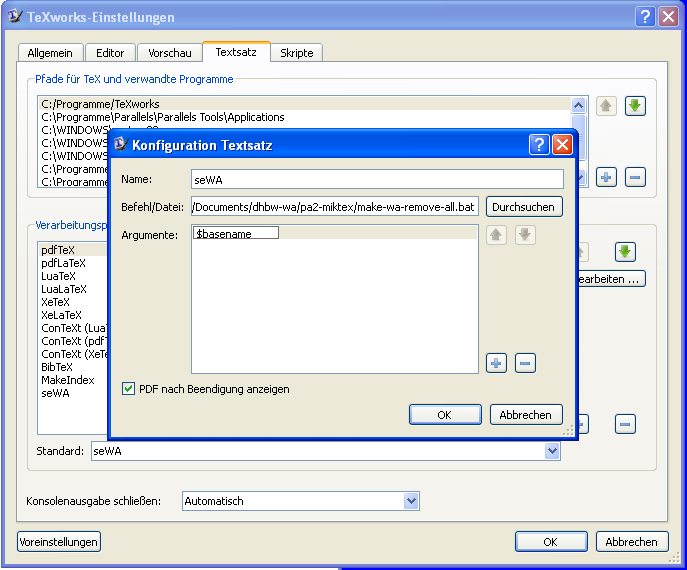
\includegraphics[width=\textwidth]{\seWaPathJpg/konfiguration-texworks.jpg}
\caption{Konfiguration von TeXworks -- Das Eintragen des Wertes  \texttt{\$basename} im Feld \textsl{Argumente}\label{texworks}}
\end{figure}

\newpage
\section{Ausdrucken des pdf-Dokuments}

Beim Ausdrucken des Dokuments (z. B. \"uber den Adobe Reader) muss unter \textsl{Seite anpassen} 
die Option \textsl{Tats\"achliche Gr\"o{\ss}e} ausgew\"ahlt werden (siehe \vref{ausdrucken}). Andernfalls werden die Einstellungen 
f\"ur das Layout der Arbeit nicht korrekt wiedergegeben. 

\begin{figure}[htbp]
\centering
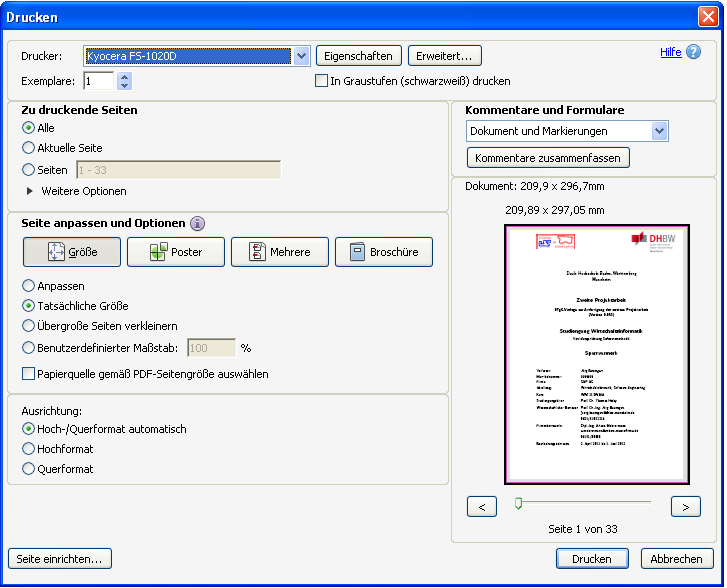
\includegraphics[width=\textwidth]{\seWaPathJpg/ausdrucken.jpg}
\caption{Ausdrucken des pdf-Dokuments -- Die Option \textsl{Tats\"achliche Gr\"o{\ss}e}\label{ausdrucken}}
\end{figure}




%Dann hoffe ich mal, dass sich mit den Vorlagen etwas anfangen lŠsst. Sie sind (absichtlich) in 
%
%einer Version 0.9, da ich an den zugehšrigen sty-Dateien weitere ErgŠnzungen vornehmen werde,
%
%um fŸr zukŸnftige Arbeiten neue komfortable Kommandos zur VerfŸgung zu stellen. 